\documentclass[a4paper,14pt]{extarticle}

\usepackage[utf8x]{inputenc}
\usepackage[T1,T2A]{fontenc}
\usepackage[russian]{babel}
\usepackage{hyperref}
\usepackage{indentfirst}
\usepackage{here}
\usepackage{array}
\usepackage{graphicx}
\usepackage{caption}
\usepackage{subcaption}
\usepackage{chngcntr}
\usepackage{amsmath}
\usepackage{amssymb}
\usepackage{pgfplots}
\usepackage{pgfplotstable}
\usepackage[left=2cm,right=2cm,top=2cm,bottom=2cm,bindingoffset=0cm]{geometry}
\usepackage{multicol}

\renewcommand{\le}{\ensuremath{\leqslant}}
\renewcommand{\leq}{\ensuremath{\leqslant}}
\renewcommand{\ge}{\ensuremath{\geqslant}}
\renewcommand{\geq}{\ensuremath{\geqslant}}
\renewcommand{\epsilon}{\ensuremath{\varepsilon}}
\renewcommand{\phi}{\ensuremath{\varphi}}

\counterwithin{figure}{section}
\counterwithin{equation}{section}
\counterwithin{table}{section}
\newcommand{\sign}[1][5cm]{\makebox[#1]{\hrulefill}} % Поля подписи и даты
\graphicspath{{pics/}} % Путь до папки с картинками
\captionsetup{justification=centering,margin=1cm}
\def\arraystretch{1.3}

\begin{document}	% начало документа

\begin{titlepage}
\begin{center}
	\textbf{Санкт-Петербургский Политехнический Университет \\Петра Великого}\\[0.3cm]
	\small Институт компьютерных наук и технологий \\[0.3cm]
	\small Кафедра компьютерных систем и программных технологий\\[4cm]
	
	\textbf{ОТЧЕТ}\\ \textbf{о лабораторной работе}\\[0.5cm]
	\textbf{<<Исследование частотных характеристик пассивных RC-цепей>>}\\[0.1cm]
	\textbf{Электротехника и Электроника}\\[10.5cm]
\end{center}

\begin{flushright}
	\begin{minipage}{0.60\textwidth}
		\begin{flushleft}
			\small \textbf{Работу выполнили студенты}\\[3mm]
			\small группа 23501/4 \hspace*{17mm} Дьячков В.В.\\[3mm]
			\small группа 23501/4 \hspace*{17mm} Ламтев А.Ю.\\[5mm]
			
			\small \textbf{Преподаватель}\\[5mm]
		 	\small \sign[3.5cm] \hspace*{8mm} к.т.н., доц. Кочетков Ю.Д.\\[0.5cm]
		\end{flushleft}
	\end{minipage}
\end{flushright}

\vfill

\begin{center}
	\small Санкт-Петербург\\
	\small \the\year
\end{center}
\end{titlepage}


\section{Цель работы}
Исследовать процессы, происхожящие в дифференцирующей и интегрирующей RC-цепях при подаче на вход однополярного прямоугольного импульса.

\section{Чертеж схемы исследуемого устройства}
\begin{figure}[h]
\centering
\begin{subfigure}[b]{0.35\textwidth}
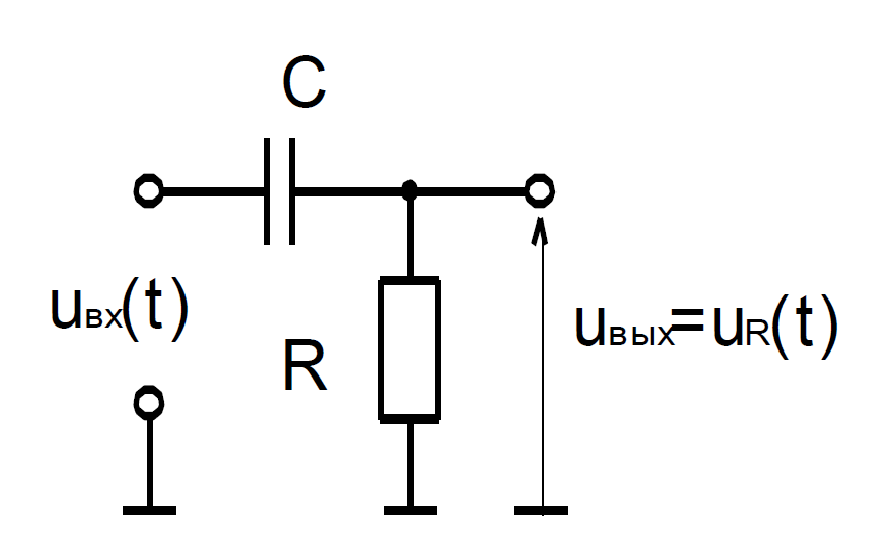
\includegraphics[scale=0.27]{diff.png}
\caption{Дифференцирующая\\ цепь}\label{figure:2.1:a}
\end{subfigure}
\begin{subfigure}[b]{0.35\textwidth}
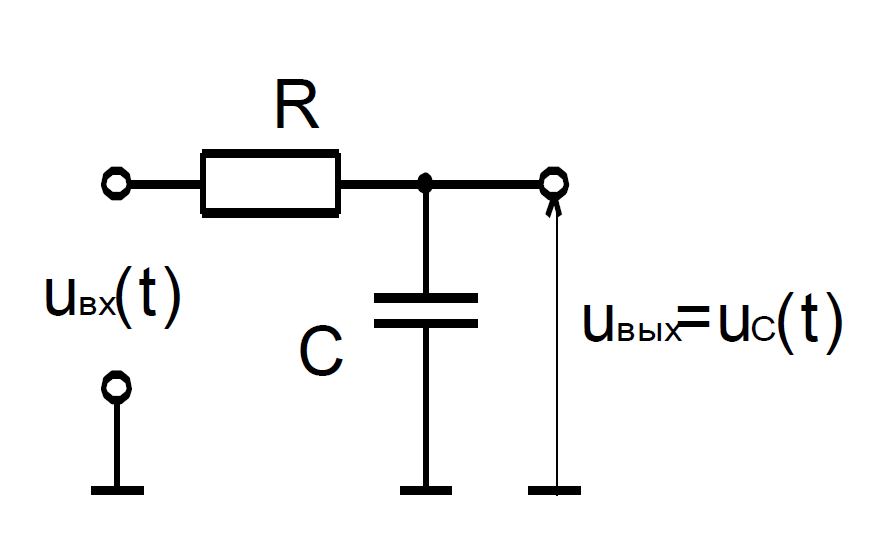
\includegraphics[scale=0.27]{int.png}
\caption{Интегрирующая\\ цепь}\label{figure:2.1:b}
\end{subfigure}
\end{figure}

На рисунке \ref{figure:2.1:a} изображена дифференцирующая RC-цепь, на \ref{figure:2.1:b} - интегрирующая RC-цепь.


\section{Исходные данные}

Исходные значения были выбраны как в таблице \ref{tabular:11}:


\begin{table}[H]
	\begin{center}
	\caption{Исходные данные}
	\def\arraystretch{1.5}
		\begin{tabular}{|c|c|c|c|c|c|c|}
			\hline 
			№ & Тип цепи & $U_\text{имп}$, B & R, кОм & С, нФ & $t_\text{имп}$, $\mu c$ & Q\\ 
			\hline 
			1 & Дифф & 10 & 10 & 0.1 & 10 & 10\\ 
			\hline 
			2 & Дифф & 10 & 10 & 1 & 10 & 10\\ 
			\hline 
			3 & Дифф & 10 & 10 & 10 & 10 & 10\\ 
			\hline 
			4 & Инт & 10 & 10 & 0.1 & 10 & 10\\ 
			\hline 
			5 & Инт & 10 & 10 & 1 & 10 & 10\\ 
			\hline 
			6 & Инт & 10 & 10 & 10 & 10 & 10\\
			\hline 
			7 & Инт & 10 & 10 & 10 & 10 & 5\\ 
			\hline 
			8 & Инт & 10 & 10 & 10 & 10 & 3\\ 
			\hline
		\end{tabular} 
	\end{center}
\end{table}

\section{Теоретические зависимости}

\section{Экспериментально снятые зависимости}


\section{Погрешности}

\subsection{Предельно допустимые погрешности}
\begin{center}
$\delta R = 0.1 = 10\%$\\
$\delta C = 0.1 = 10\%$\\
\end{center}

  
\section{Выводы}
Все классно

\end{document}
